\begin{titlepage}
    \tikzset{help lines/.style=thick}
    \begin{tikzpicture}[overlay, remember picture]
        \filldraw[fill = titlegreendark!50!white, line width = 0pt, titlegreendark!50!white] (current page.south west) rectangle +(\paperwidth,\paperheight);
        \def\rectanglepath#1{\filldraw[fill = titlegreendark, line width = 0pt, titlegreendark, rotate = 45] #1 rectangle +(3,3);}
        \foreach\i in {-36,-30,...,18}{\foreach\j in {-36,-30,...,18}{\rectanglepath{(\i,\j)}\rectanglepath{(\i+3,\j+3)}}}
        \draw[help lines, step=.3cm, opacity = .02] (-30,-30) grid (30,30);
    \end{tikzpicture}
    \begin{tikzpicture}[overlay, remember picture, opacity = .1]
        \foreach \x in {1,...,500}{
                \pgfmathrandominteger{\a}{-1000}{500}
                \pgfmathrandominteger{\b}{-1000}{500}
                \pgfpathcircle{\pgfpoint{+\a pt}{+\b pt}}{+3pt}
                \color{titlegreendark!70!black}
                \pgfusepath{fill}
            }
        \end{tikzpicture}
    \begin{tikzpicture}[overlay, remember picture]
        \node[opacity = .2] at ([xshift = .5\paperwidth, yshift = -.5\paperheight]current page.north west){
            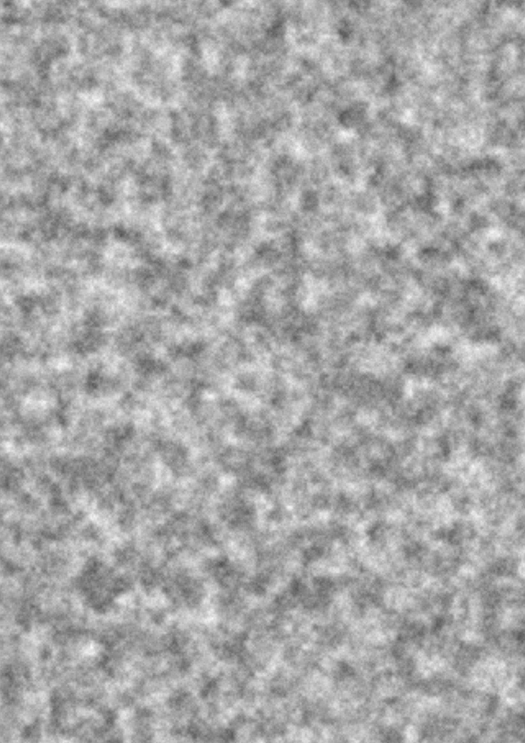
\includegraphics[width=\paperwidth]{title-bg.png}
        };
        \filldraw [fill = white, opacity = .8, thick] ([xshift = .2\paperwidth, yshift = -.25\paperheight]current page.north west) rectangle ([xshift = -.2\paperwidth, yshift = -.5\paperheight]current page.north east);
        \node at ([xshift = .5\paperwidth, yshift = -.375\paperheight]current page.north west) {\Huge\bfseries \parbox[c]{10em}{\centering 高等实分析引论\\ \bigskip\sffamily\large Gerald B. Folland~~著}};
    \end{tikzpicture}
\end{titlepage}